First we run a normal wordcount job on the cluster and use Memmetric to monitor it. In this wordcount job, no memory is used for storage therefore a presumable result would be a straight line close to the x-axis in the real-time monitor. However, the running result is shown in Fig. \ref{ref:baseline.png}.
\begin{figure}[ht]
  \centering
    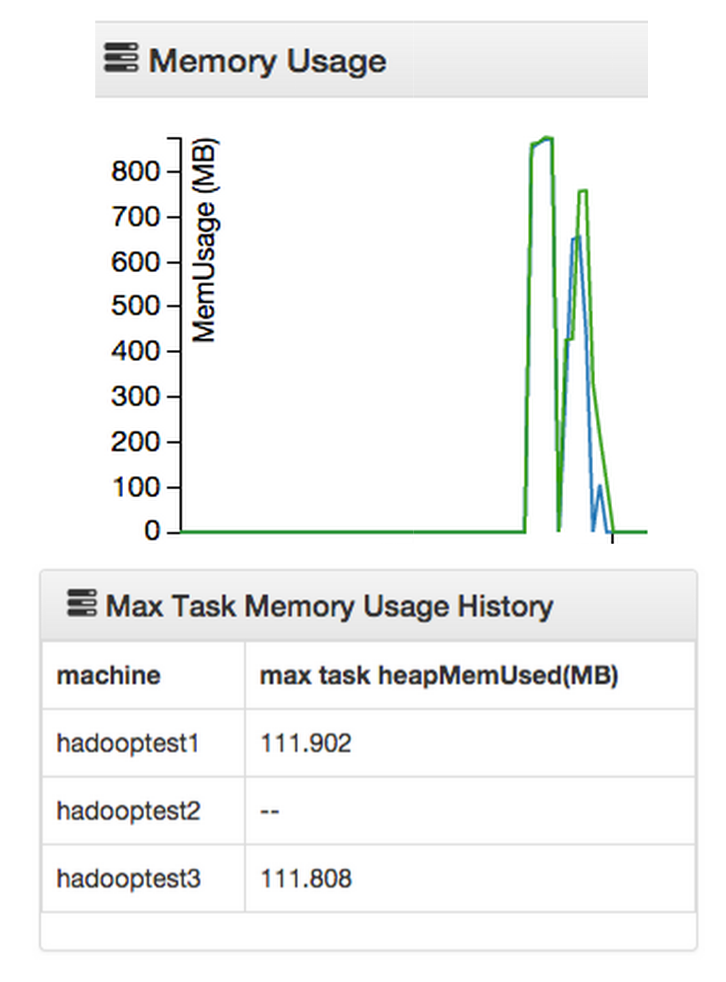
\includegraphics[width=2.1in]{image/baselinemodified.png}
    \caption{Historical memory usage of normal wordcount job.}
    \label{ref:baseline.png}
\end{figure}
\par
In the process of the above job, one of the tasks failed because there is not enough disk space, so there is a sharp cave in the middle of the curve.
In addition to this phenomenon, what is mostly interesting is the beginning of the job: even though there is no memory used to store intermediate data, the initial memory usage of a task is around 100 MB.
From the real-time monitor, the job runs about 3 minutes, and during the execution procedure of the Hadoop job, the curve is roughly flat.